%************************************************
\chapter{Black-box Model}\label{ch:Blackbox}
%************************************************

We speak of a black-box model when we the user are not aware of the inner workings of the system, like the name suggests we are
in the dark on how the system works, for all we know is that given a input the black-box returns a output according to the systems 
specifications. 

A well known example of a black-box system are neural networks, they start of with a problem and exampels on how to solve it, 
during several iterations, the network improves itself and is able to solve the problem
more efficiently and accurately. While we know what problem the neural network is solving, if we would step into the code, 
we would not be able to understand the structure and reasoning behind it. For us humans, it is impossible to understand how
all the neurons interact with each other and for what specific reason. \cite{NeuralNetworks}.

However, since we want to compare black-box and white-box model, we need to do that on the same systems, so
we cannot choose black-box system for our experiments, since the white-box model could not produce data in this case.
We solve this problem by choosing a commonly available white-box system, such as xz, but even though we have acess to the code, we dont use
that knowledge and look at the system from a black-box perspective.

\section{Disadvantages of black-box model}
When using the black-box model we encouter two major challanges, combinatorial explosion and collinear features, both need to be
handled carefully in order to build an accurate performance-influence model.

\paragraph{Combinatorial Explosion}
One of the larger problems we face when using black-box models is the issue of combinatorial explosion, 
which refers to the effect that when features increase linearly, the number of possible configuration and thus system variants,
 increase exponentially \cite{Combinatorial-explosion}.

Suppose we have a configurable system where each feature is a binary option that you can either turn on or off. We also define 
that in this system each feature is completely independent of another, i.e. the system has no constraints and turning a feature on or off
has no affect on other features. The number of unique configurations this system can produce is $2^n$, where $2$ refers to
the type of feature options allowed, binary in our case and $n$ denotes the number of features. In Figure \ref{fig:Combinatorial-Explosion-Graph}
we can see the effects of combinatorial explosion in such a system, since our system provides 15 features, we can see that the number of 
unique configurations equal to $32768$. 

\begin{figure}[h]
    \centering
    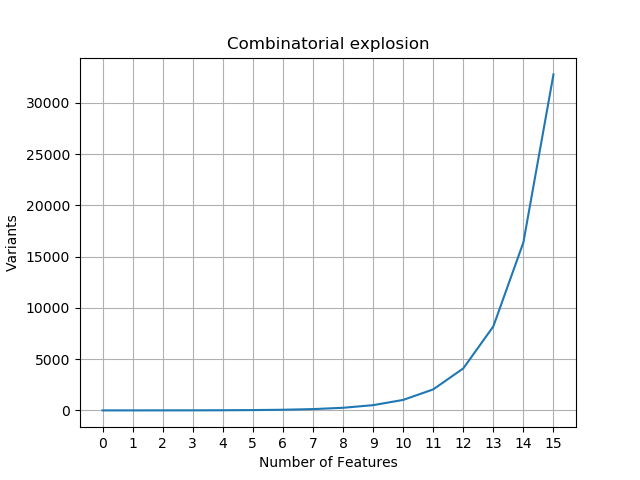
\includegraphics[scale=0.6]{gfx/Combinatorial_explosion_graph.png}
    \caption{Combinatorial Explosion Graph}
    \label{fig:Combinatorial-Explosion-Graph}
\end{figure}

Here is the problem, because 15 features is by no means a lot compared to the ammount of functions a real world systems like the
linux kernel contains. All these different features might interact with each other in different ways, and for very small systems,
we can certainly brute-force our way by benchmarking all possible configuration, however this does not scale, it is already not feasible for systems that
have more then 16 features and therefore over $100.000$ configurations. For this reason, we cannot fully expore the entire configuration space 
and therefore need to select a subset that represent the system with a high accuracy. To do that state of the art black-box model use sampling
strategies to find a suitable subset, such as, pair-wise sampling, most-enabled-disabled and random sampling. A in depht comparison
between state of the art sampling strategies has been done by Medeiros et.al \cite{sampling-strategies}.

\paragraph{Colinear Features}\label{ColinearF}
Another problem for our black-box model arises when we have features that are correlated with each other, we call such features collinear.
Let's make an example and revisit our code from Chapter \ref{ch:performance-influence-models} Algorithm \ref{alg:performanceExample} and let's
 extend it with the condition $c \leftrightarrow d$. We add this new condition from Algorithm \ref{alg:Colinear} in Algorithm 
\ref{alg:performanceExample} after line 2.

\begin{algorithm}
    \caption{Colinear Features \label{alg:Colinear}}
    \begin{algorithmic}[1]

    \If{$(c \textit{ and }  \lnot d) or (\lnot c \textit{ and } d)$} 
        \State $c,d \gets False$
    \EndIf

    \end{algorithmic}
    \end{algorithm}

Now, if our configuration does not contain c and d, the code in line 9 and 11 is unreachable. These colinear features make it difficult 
for our black-box model to correctly assign time to each feature, because if we are unaware of the inner workings, we might mistakenly think
that the increase in time when feature c and d are activated is due to the interaction between them, but in fact we see in line
15 that they do not interact at all. % Maybe elastic net

\section{Collecting data}

Let us now proceed on how we collect data. First, we analyze the configuration space using our feature model introduced in Chapter \ref{ch:Feature Model}
and decide on the set of features we want to analyze. To deal with the effects of combinatorial explosion, we select a subset of the entire
configuration space and analyze it using a brute force approach, rather using sampling strategies which would exceed the scope of this
thesis.

In addition, we will only use valid configurations that satisfy the constraints of our feature model, to mitigate
the influence that colinear features have or our model.


\section{Creating a Performance-Influence Model using Multiple Linear Regression}
We use our black-box model by feeding it inputs and meassuring the time it takes the system to produce a output. From this 
very limited set of data, we now need to bulid our performance-influence model, which we do by using multiple linear regression.
We use multiple linear regression beacause the formular we learn can be understood by us humans, unlike other approaches like neural networks.
Moreover, to use multiple linear regression, we do not need to know anything about the inner workings of the system,
which benefits our black-box model. \cite{Linear-Regression-Performance}

We use the following formular of linear regression for matrices\cite{Linear-Regression-Performance}:

\begin{align*}
        y &= \beta_0 + \beta_1 x_1 + \beta_2 x_2 ... \beta_n x_n + \epsilon   \\
        y &= X \beta + \epsilon
\end{align*}


Where $y$ is called dependendent variable and $X$ is called independent variable $y$ in our case is a vector with n elements containing
the output of our black-box model, i.e. the time meassurement generated for each feature configuration in our feature set. What we
are intrested in are the values of the coefficents $\beta$, since they quantify the influence of each feature or feature interaction
on to the whole system. In addition, $\beta_0$ denotes the intercept, which for us represents the influence of the base code, meaning
the part of the code that gets exectued regardless of the selected feature configuration.
Our independent variable $X$ is a $n \times m$ martrix, where $n$ is the number of configurations used and $m$ the powerset of all
features. The reason we use a powerset here is to model all feature interactions in our matrix.
The value of each feature in the matrix is either $1$ if the feature is selected, or $0$ if its not. If we have numerical features with $l$
different options, we split this features into $l$ binary features and encode them as an alternative group in our feature model.
For all our meassurements we also have a possible error represented by $\epsilon$. \cite{Linear-Regression}

%To Do superset features

